\documentclass{article}
\usepackage{tikz}
\usetikzlibrary{shapes, backgrounds}

\begin{document}

\begin{center}
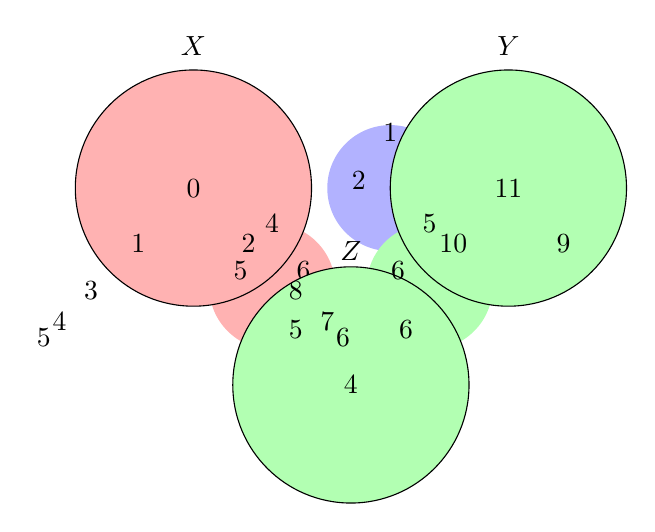
\begin{tikzpicture}
    % Set X
    \draw (0,0) circle (1.5);
    \node at (0, 1.8) {$X$};
    \node at (0, 0) {0};
    \node at (-0.7, -0.7) {1};
    \node at (0.7, -0.7) {2};
    \node at (-1.3, -1.3) {3};
    \node at (1.3, -1.3) {8};
    \node at (-1.7, -1.7) {4};
    \node at (1.7, -1.7) {7};
    \node at (-1.9, -1.9) {5};
    \node at (1.9, -1.9) {6};

    % Set Y
    \draw (4,0) circle (1.5);
    \node at (4, 1.8) {$Y$};
    \node at (4, 0) {11};
    \node at (3.3, -0.7) {10};
    \node at (4.7, -0.7) {9};

    % Set Z
    \draw (2, -2.5) circle (1.5);
    \node at (2, -0.8) {$Z$};
    \node at (2, -2.5) {4};
    \node at (1.3, -1.8) {5};
    \node at (2.7, -1.8) {6};

    % Intersection X and Y
    \begin{scope}[on background layer]
        \fill[blue!30] (0,0) circle (1.5);
        \fill[blue!30] (4,0) circle (1.5);
        \fill[blue!30] (2.5,0) circle (0.8);
        \node at (2.5, 0.7) {1};
        \node at (2.1, 0.1) {2};
        \node at (2.9, 0.1) {3};
    \end{scope}

    % Intersection X and Z
    \begin{scope}[on background layer]
        \fill[red!30] (0,0) circle (1.5);
        \fill[red!30] (2, -2.5) circle (1.5);
        \fill[red!30] (1, -1.25) circle (0.8);
        \node at (1, -0.45) {4};
        \node at (0.6, -1.05) {5};
        \node at (1.4, -1.05) {6};
    \end{scope}

    % Intersection Y and Z
    \begin{scope}[on background layer]
        \fill[green!30] (4,0) circle (1.5);
        \fill[green!30] (2, -2.5) circle (1.5);
        \fill[green!30] (3, -1.25) circle (0.8);
        \node at (3, -0.45) {5};
        \node at (2.6, -1.05) {6};
    \end{scope}

\end{tikzpicture}
\end{center}

\end{document}
